%%%%%%%%%%%%%%%%%%%%%%
%% Document details %%
%%%%%%%%%%%%%%%%%%%%%%

% Paper title
\title{Dynamic Autotuning\\of Algorithmic Skeletons}

% Author
\author{Chris Cummins}

%%%%%%%%%%%%%%%%%%%%%%%%%
%% Document and Layout %%
%%%%%%%%%%%%%%%%%%%%%%%%%

% Fix for multiple "No room for a new \dimen" errors.
%
% See: http://tex.stackexchange.com/questions/38607/no-room-for-a-new-dimen
%
\usepackage{etex}

\usepackage{booktabs}

\usepackage[utf8]{inputenc}

% Make internal macro definitions accessible,
% e.g. \@title, \@date \@author.
\makeatletter

% Multi-column support.
\usepackage{multicol}

% A useful package which includes macros like \ifdef{}{}{}:
%
\usepackage{etoolbox}

% Uncomment the following line to remove column separation:
%
%\setlength{\columnsep}{5mm}


% Set chapter and section numbering depth:
%
\setcounter{secnumdepth}{2}


%%%%%%%%%%%%%%%%%%%%%%%%%%%%%%%%%
%% Bibliography and Appendices %%
%%%%%%%%%%%%%%%%%%%%%%%%%%%%%%%%%
\usepackage[%
    backend=biber,
    style=numeric-comp,  % numerical-compressed
    sorting=none,        % nty,nyt,nyvt,anyt,anyvt,ynt,ydnt,none
    sortcites=true,      % sort \cite{b a d c}: true,false
    block=none,          % space between blocks: none,space,par,nbpar,ragged
    indexing=false,      % indexing options: true,false,cite,bib
    citereset=none,      % don't reset cites
    isbn=false,          % print ISBN?
    url=false,           % print URL?
    doi=false,           % print DOI?
    natbib=true,         % natbib compatability
  ]{biblatex}

% Reduce the font size of the bibliography:
% \renewcommand{\bibfont}{\normalfont\scriptsize}

% Determine which BibTeX file to use:
%
% If available, use my Mendeley BibTex library, located in the home
% directory. Note that this is a relative path and will break if
% either this file or the BibTex library are moved. If the library is
% not present, use the local refs.bib file.
\newcommand{\BibResourceGlobal}{../../../../library.bib}
\newcommand{\BibResourceLocal}{refs.bib}

\IfFileExists{\BibResourceGlobal}
  {\newcommand{\BibResource}{\BibResourceGlobal}}
  {\newcommand{\BibResource}{\BibResourceLocal}}

\addbibresource{\BibResource}

% Appendix package. Documentation:
%
%  http://mirror.ox.ac.uk/sites/ctan.org/macros/latex/contrib/appendix/appendix.pdf
%
% Package options:
%
% toc      - Put a header (e.g., `Appendices') into the Table of Contents
%            (the ToC) before listing the appendices. (This is done by
%            calling the \addappheadtotoc command.)
% page     - Puts a title (e.g., `Appendices') into the document at the
%            point where the appendices environment is begun. (This is
%            done by calling the \appendixpage command.)
% title    - Adds a name (e.g., `Appendix') before each appendix title in
%            the body of the document. The name is given by the value
%            of \appendixname. Note that this is the default behaviour
%            for classes that have chapters.
% titletoc - Adds a name (e.g., `Appendix') before each appendix listed
%            in the ToC. The name is given by the value
%            of \appendixname.
% header   - Adds a name (e.g., `Appendix') before each appendix in page
%            headers.  The name is given by the value
%            of \appendixname. Note that this is the default behaviour
%            for classes that have chapters.
\usepackage[title, titletoc]{appendix}


%%%%%%%%%%%%%%%%%%%%%%%%%%%%%%%%%%%%%
%% Figures, footnotes and listings %%
%%%%%%%%%%%%%%%%%%%%%%%%%%%%%%%%%%%%%

%\usepackage{float}
%\restylefloat{figure}

% Use bold ``(Figure|Table|Listing)'' caption text.
%\usepackage[margin=1cm]{caption}

% Set the font for captions.
%\renewcommand{\captionfont}{\footnotesize}
% Set the font for caption labels.
%\renewcommand{\captionlabelfont}{\footnotesize\bf}

% Use arabic numbers for footnote.
%\renewcommand{\thefootnote}{\arabic{footnote}}

% Ensure that footnotes always appear at the bottom of pages.
%\usepackage[bottom]{footmisc}

% Reset the footnote counter on every page.
%\usepackage{perpage}
%\MakePerPage{footnote}

% Pre-requisites for rendering upquotes in listings package.
\usepackage[T1]{fontenc}
\usepackage{lmodern}
\usepackage{textcomp}

% Pseudo-code listings.
\usepackage{algorithm}
\usepackage{algpseudocode}
\newcommand{\Break}{\State \textbf{break} }
\algblockdefx[Loop]{Loop}{EndLoop}[1][]{\textbf{Loop} #1}{\textbf{End
    Loop}}

\algrenewcommand\ALG@beginalgorithmic{\footnotesize}

% Code listings.
\usepackage{listings}

% Set \ttfamily to use courier fonts.
%
% See: http://tex.stackexchange.com/a/33686
%
\usepackage{courier}

\lstset{frame=bt,                    % Add top and bottom frame lines
        breaklines=true,             % Force line wrapping
        captionpos=b,                % Place caption below listing
        numbers=left,                % Add left-side line numbers
        basicstyle=\scriptsize\ttfamily, % Set font size and type
        showstringspaces=false,      % Don't show visible whitespace
        numberstyle=\tiny,
        upquote=true,                % Use upright quotes, not curly
        commentstyle=\bfseries}      % Embolden comments

% Use (*@ @*) to escape LaTeX commands within listings.
\lstset{escapeinside={(*@}{@*)}}

% Add 10pt space between chapters in TOC listings entries:
%\let\Chapter\chapter
%\def\chapter{\addtocontents{lol}{\protect\addvspace{10pt}}\Chapter}

% Add JavaScript support to listings. See:
%
%     http://tex.stackexchange.com/a/89576
%
\lstdefinelanguage{JavaScript}{
  keywords={
    break,
    case,
    catch,
    catch,
    do,
    else,
    false,
    function,
    if,
    in,
    new,
    null,
    return,
    switch,
    true,
    typeof,
    var,
    while}
  keywordstyle=\bfseries,
  ndkeywords={
    boolean,
    class,
    export,
    implements,
    import,
    this,
    throw}
  ndkeywordstyle=\bfseries,
  sensitive=false,
  comment=[l]{//},
  morecomment=[s]{/*}{*/},
  morestring=[b]',
  morestring=[b]"
}

% Add Clojure support to listings. See:
%
%     http://alexott.blogspot.co.uk/2010/01/clojure-latex.html
%
\lstdefinelanguage{Clojure}{morekeywords={
    *,
    *1,
    *2,
    *3,
    *agent*,
    *allow-unresolved-vars*,
    *assert*,
    *clojure-version*,
    *command-line-args*,
    *compile-files*,
    *compile-path*,
    *e,
    *err*,
    *file*,
    *flush-on-newline*,
    *in*,
    *macro-meta*,
    *math-context*,
    *ns*,
    *out*,
    *print-dup*,
    *print-length*,
    *print-level*,
    *print-meta*,
    *print-readably*,
    *read-eval*,
    *source-path*,
    *use-context-classloader*,
    *warn-on-reflection*,
    +,
    -,
    ->,
    ->>,
    ..,
    /,
    :else,
    <,
    <=,
    =,
    ==,
    >,
    >=,
    @,
    accessor,
    aclone,
    add-classpath,
    add-watch,
    agent,
    agent-errors,
    aget,
    alength,
    alias,
    all-ns,
    alter,
    alter-meta!,
    alter-var-root,
    amap,
    ancestors,
    and,
    apply,
    areduce,
    array-map,
    aset,
    aset-boolean,
    aset-byte,
    aset-char,
    aset-double,
    aset-float,
    aset-int,
    aset-long,
    aset-short,
    assert,
    assoc,
    assoc!,
    assoc-in,
    associative?,
    atom,
    await,
    await-for,
    await1,
    bases,
    bean,
    bigdec,
    bigint,
    binding,
    bit-and,
    bit-and-not,
    bit-clear,
    bit-flip,
    bit-not,
    bit-or,
    bit-set,
    bit-shift-left,
    bit-shift-right,
    bit-test,
    bit-xor,
    boolean,
    boolean-array,
    booleans,
    bound-fn,
    bound-fn*,
    butlast,
    byte,
    byte-array,
    bytes,
    cast,
    char,
    char-array,
    char-escape-string,
    char-name-string,
    char?,
    chars,
    chunk,
    chunk-append,
    chunk-buffer,
    chunk-cons,
    chunk-first,
    chunk-next,
    chunk-rest,
    chunked-seq?,
    class,
    class?,
    clear-agent-errors,
    clojure-version,
    coll?,
    comment,
    commute,
    comp,
    comparator,
    compare,
    compare-and-set!,
    compile,
    complement,
    concat,
    cond,
    condp,
    conj,
    conj!,
    cons,
    constantly,
    construct-proxy,
    contains?,
    count,
    counted?,
    create-ns,
    create-struct,
    cycle,
    dec,
    decimal?,
    declare,
    def,
    definline,
    defmacro,
    defmethod,
    defmulti,
    defn,
    defn-,
    defonce,
    defprotocol,
    defstruct,
    deftype,
    delay,
    delay?,
    deliver,
    deref,
    derive,
    descendants,
    destructure,
    disj,
    disj!,
    dissoc,
    dissoc!,
    distinct,
    distinct?,
    do,
    do-template,
    doall,
    doc,
    dorun,
    doseq,
    dosync,
    dotimes,
    doto,
    double,
    double-array,
    doubles,
    drop,
    drop-last,
    drop-while,
    empty,
    empty?,
    ensure,
    enumeration-seq,
    eval,
    even?,
    every?,
    false,
    false?,
    ffirst,
    file-seq,
    filter,
    finally,
    find,
    find-doc,
    find-ns,
    find-var,
    first,
    float,
    float-array,
    float?,
    floats,
    flush,
    fn,
    fn?,
    fnext,
    for,
    force,
    format,
    future,
    future-call,
    future-cancel,
    future-cancelled?,
    future-done?,
    future?,
    gen-class,
    gen-interface,
    gensym,
    get,
    get-in,
    get-method,
    get-proxy-class,
    get-thread-bindings,
    get-validator,
    hash,
    hash-map,
    hash-set,
    identical?,
    identity,
    if,
    if-let,
    if-not,
    ifn?,
    import,
    in-ns,
    inc,
    init-proxy,
    instance?,
    int,
    int-array,
    integer?,
    interleave,
    intern,
    interpose,
    into,
    into-array,
    ints,
    io!,
    isa?,
    iterate,
    iterator-seq,
    juxt,
    key,
    keys,
    keyword,
    keyword?,
    last,
    lazy-cat,
    lazy-seq,
    let,
    letfn,
    line-seq,
    list,
    list*,
    list?,
    load,
    load-file,
    load-reader,
    load-string,
    loaded-libs,
    locking,
    long,
    long-array,
    longs,
    loop,
    macroexpand,
    macroexpand-1,
    make-array,
    make-hierarchy,
    map,
    map?,
    mapcat,
    max,
    max-key,
    memfn,
    memoize,
    merge,
    merge-with,
    meta,
    method-sig,
    methods,
    min,
    min-key,
    mod,
    monitor-enter,
    monitor-exit,
    name,
    namespace,
    neg?,
    new,
    newline,
    next,
    nfirst,
    nil,
    nil?,
    nnext,
    not,
    not-any?,
    not-empty,
    not-every?,
    not=,
    ns,
    ns-aliases,
    ns-imports,
    ns-interns,
    ns-map,
    ns-name,
    ns-publics,
    ns-refers,
    ns-resolve,
    ns-unalias,
    ns-unmap,
    nth,
    nthnext,
    num,
    number?,
    odd?,
    or,
    parents,
    partial,
    partition,
    pcalls,
    peek,
    persistent!,
    pmap,
    pop,
    pop!,
    pop-thread-bindings,
    pos?,
    pr,
    pr-str,
    prefer-method,
    prefers,
    primitives-classnames,
    print,
    print-ctor,
    print-doc,
    print-dup,
    print-method,
    print-namespace-doc,
    print-simple,
    print-special-doc,
    print-str,
    printf,
    println,
    println-str,
    prn,
    prn-str,
    promise,
    proxy,
    proxy-call-with-super,
    proxy-mappings,
    proxy-name,
    proxy-super,
    push-thread-bindings,
    pvalues,
    quot,
    rand,
    rand-int,
    range,
    ratio?,
    rational?,
    rationalize,
    re-find,
    re-groups,
    re-matcher,
    re-matches,
    re-pattern,
    re-seq,
    read,
    read-line,
    read-string,
    recur,
    reduce,
    ref,
    ref-history-count,
    ref-max-history,
    ref-min-history,
    ref-set,
    refer,
    refer-clojure,
    reify,
    release-pending-sends,
    rem,
    remove,
    remove-method,
    remove-ns,
    remove-watch,
    repeat,
    repeatedly,
    replace,
    replicate,
    require,
    reset!,
    reset-meta!,
    resolve,
    rest,
    resultset-seq,
    reverse,
    reversible?,
    rseq,
    rsubseq,
    second,
    select-keys,
    send,
    send-off,
    seq,
    seq?,
    seque,
    sequence,
    sequential?,
    set,
    set!,
    set-validator!,
    set?,
    short,
    short-array,
    shorts,
    shutdown-agents,
    slurp,
    some,
    sort,
    sort-by,
    sorted-map,
    sorted-map-by,
    sorted-set,
    sorted-set-by,
    sorted?,
    special-form-anchor,
    special-symbol?,
    split-at,
    split-with,
    str,
    stream?,
    string?,
    struct,
    struct-map,
    subs,
    subseq,
    subvec,
    supers,
    swap!,
    symbol,
    symbol?,
    sync,
    syntax-symbol-anchor,
    take,
    take-last,
    take-nth,
    take-while,
    test,
    the-ns,
    throw,
    time,
    to-array,
    to-array-2d,
    trampoline,
    transient,
    tree-seq,
    true,
    true?,
    try,
    type,
    unchecked-add,
    unchecked-dec,
    unchecked-divide,
    unchecked-inc,
    unchecked-multiply,
    unchecked-negate,
    unchecked-remainder,
    unchecked-subtract,
    underive,
    unquote,
    unquote-splicing,
    update-in,
    update-proxy,
    use,
    val,
    vals,
    var,
    var-get,
    var-set,
    var?,
    vary-meta,
    vec,
    vector,
    vector?,
    when,
    when-first,
    when-let,
    when-not,
    while,
    with-bindings,
    with-bindings*,
    with-in-str,
    with-loading-context,
    with-local-vars,
    with-meta,
    with-open,
    with-out-str,
    with-precision,
    xml-seq,
    zero?,
    zipmap
  },
  sensitive,
  alsodigit=-,
  morecomment=[l];,
  morestring=[b]"
}[keywords,comments,strings]


%%%%%%%%%%%%%%%%%%%%%%%%
%% Graphics and maths %%
%%%%%%%%%%%%%%%%%%%%%%%%
\usepackage{amsmath}

% Additional amsmath symbols, see:
%
% http://texblog.org/2007/08/27/number-sets-prime-natural-integer-rational-real-and-complex-in-latex/
%
\usepackage{amssymb}

\usepackage{graphicx}
\usepackage{mathtools}
\usepackage{tikz}
\usepackage{tikz-qtree}

% Provide bold font face in maths.
\usepackage{bm}

\usepackage{subcaption}
\expandafter\def\csname ver@subfig.sty\endcsname{}

% Define an 'myalignat' command which behave as 'alignat' without the
% vertical top and bottom padding. See:
%     http://www.latex-community.org/forum/viewtopic.php?f=5&t=1890
\newenvironment{myalignat}[1]{%
  \setlength{\abovedisplayskip}{-.7\baselineskip}%
  \setlength{\abovedisplayshortskip}{\abovedisplayskip}%
  \start@align\z@\st@rredtrue#1
}%
{\endalign}

% Define additional operators:
\DeclareMathOperator*{\argmin}{arg\,min}
\DeclareMathOperator*{\argmax}{arg\,max}

% Skeleton operators.
\DeclareMathOperator*{\map}{Map}
\DeclareMathOperator*{\reduce}{Reduce}
\DeclareMathOperator*{\scan}{Scan}
\DeclareMathOperator*{\stencil}{Stencil}
\DeclareMathOperator*{\zip}{Zip}
\DeclareMathOperator*{\allpairs}{All\,Pairs}

% Maths plots using pgfplots, see:
%
%     http://pgfplots.sourceforge.net/pgfplots.pdf
%
\usepackage{pgfplots}

% Gantt charts using pgfgantt, see:
%
%     http://www.ctan.org/pkg/pgfgantt
%
\usepackage{pgfgantt}

% Fix milestone aspect ratio by defining a custom element.
\newganttchartelement*{mymilestone}{
  mymilestone/.style={
    shape=diamond,
    inner sep=2pt,
    draw=black,
    top color=black,
    bottom color=black,
  }
}

% Tikz flowchart configuration.
\usetikzlibrary{shapes,arrows,shadows,fit,backgrounds}
\tikzstyle{decision} = [diamond,
                        draw,
                        text width=4.5em,
                        text badly centered,
                        node distance=3cm,
                        inner sep=0pt]
\tikzstyle{block}    = [rectangle,
                        draw,
                        text width=5em,
                        text centered,
                        node distance=3cm,
                        minimum height=4em,
                        inner sep=.2cm]
\tikzstyle{line}     = [draw, -latex']

% Add dirtree picture style, see:
%
%     http://tex.stackexchange.com/a/34268
%
\newcount\dirtree@lvl
\newcount\dirtree@plvl
\newcount\dirtree@clvl
\def\dirtree@growth{%
  \ifnum\tikznumberofcurrentchild=1\relax
    \global\advance\dirtree@plvl by 1
    \expandafter\xdef\csname dirtree@p@\the\dirtree@plvl\endcsname{\the\dirtree@lvl}
  \fi
  \global\advance\dirtree@lvl by 1\relax
  \dirtree@clvl=\dirtree@lvl
  \advance\dirtree@clvl by -\csname dirtree@p@\the\dirtree@plvl\endcsname
  \pgf@xa=0.33cm\relax
  \pgf@ya=-\baselineskip\relax
  \pgf@ya=\dirtree@clvl\pgf@ya
  \pgftransformshift{\pgfqpoint{\the\pgf@xa}{\the\pgf@ya}}%
  \ifnum\tikznumberofcurrentchild=\tikznumberofchildren
    \global\advance\dirtree@plvl by -1
  \fi
}
\tikzset{
  dirtree/.style={
    growth function=\dirtree@growth,
    every node/.style={anchor=north},
    every child node/.style={anchor=west},
    edge from parent path={(\tikzparentnode\tikzparentanchor) |- (\tikzchildnode\tikzchildanchor)}
  }
}

% UML sequence diagram macros, see:
%
%     https://code.google.com/p/pgf-umlsd/
%
% Options:
%
%     underline - Underline object names
%
\usepackage[underline=false]{pgf-umlsd}

% Support for SVG graphics.
%
% NOTE that you must pass the "--shell-escape" argument to pdflatex to
% compile. NOTE also that images *MUST* be placed within the graphics
% path.
\usepackage{svg}
\graphicspath{{img/}}

%%%%%%%%%%%%%%%%%%%%%%
%% Tables and lists %%
%%%%%%%%%%%%%%%%%%%%%%

%\usepackage{enumitem}
%\setenumerate{itemsep=0pt}

% Use no left margin for lists:
%\setlist{leftmargin=*}

\usepackage{longtable}

% Define column types L, C, R with known text justification and fixed
% widths:
\usepackage{array}
\newcolumntype{L}[1]{>{\raggedright\let\newline\\\arraybackslash\hspace{0pt}}m{#1}}
\newcolumntype{C}[1]{>{\centering\let\newline\\\arraybackslash\hspace{0pt}}m{#1}}
\newcolumntype{R}[1]{>{\raggedleft\let\newline\\\arraybackslash\hspace{0pt}}m{#1}}


%%%%%%%%%%%%%%%%%%%%%%%%%%%%%
%% Typesetting and symbols %%
%%%%%%%%%%%%%%%%%%%%%%%%%%%%%

% Adjustable font sizes in \Verbatim{}
\usepackage{fancyvrb}

%\usepackage{titlesec}
% Set section and paragraph heading fonts:
%\titleformat*{\section}{\Large\bfseries}
%\titleformat*{\subsection}{\normalsize\bfseries}
%\titleformat*{\subsubsection}{\normalsize}
%\titleformat*{\paragraph}{\large\bfseries}
%\titleformat*{\subparagraph}{\large\bfseries}

% Set section heading margins. Usage:
% \titlespacing*{<command>}{<left>}{<before>}{<after>}
%\titlespacing*{\section}{0pt}{.6em}{.3em}
%\titlespacing*{\subsection}{0pt}{.6em}{.2em}

% Set paragraph indentation size. Default is 15pt.
%\setlength{\parindent}{10pt}

% The line spacing can be globally set using \linespread:
%
% \linespread{1.2}

% Add a command \hr{} which will draw a horizontal rule the width of
% the text.
%
\newcommand{\hr}{\noindent\makebox[\linewidth]{\rule{\textwidth}{0.2pt}}}

% Add a command \br{} which will create a horizontal space of exactly
% one line height.
%
\newcommand{\br}{\hspace{\baselineskip}}

% Define a command to allow word breaking.
\newcommand*\wrapletters[1]{\wr@pletters#1\@nil}
\def\wr@pletters#1#2\@nil{#1\allowbreak\if&#2&\else\wr@pletters#2\@nil\fi}

% Define a command to create centred page titles.
\newcommand{\centredtitle}[1]{
  \begin{center}
    \large
    \vspace{0.9cm}
    \textbf{#1}
  \end{center}}

% Support hyperlinks using the \hyperref, \url and \href
% macros. Usage:
%
%    \hyperref[label_name]{''link text''}
%
%    \url{<my_url>}
%
%    \href{<my_url>}{<description>}
%
\usepackage{hyperref}

% Disable colored borders of links, cross-references etc in PDF output
\hypersetup{pdfborder={0 0 0}}

% Provide generic commands \degree, \celsius, \perthousand, \micro
% and \ohm which work both in text and maths mode.
\usepackage{gensymb}

%%%%%%%%%%%%%%%%%%%%%%%%%%%%%%%%%
%% Placeholder text generation %%
%%%%%%%%%%%%%%%%%%%%%%%%%%%%%%%%%

% Use either \blindtext or \libpsum to generate placeholder text. Also
% note the macros \blinditemize, \blindenumerate, \blinddescription.
\usepackage[english]{babel}
\usepackage{blindtext}
\usepackage{lipsum}


%%%%%%%%%%
%% Body %%
%%%%%%%%%%
\begin{document}

% \noindent
% \textit{Abstract: %
% a
% }

%\maketitle

\section{SkelCL}

SkelCL\footnote{\url{http://skelcl.uni-muenster.de}} is an object
oriented C++ library that provides OpenCL implementations of data
parallel algorithmic skeletons for heterogeneous parallelism: Map,
Reduce, Scan, Zip, Stencil, and AllPairs. Skeletons are parameterised
with muscle functions by the user, which are compiled into OpenCL
kernels for execution on device hardware. The Vector and Matrix
container types transparently handle communication between the host
and device memory, and can be distributed for multi-GPU execution.

Each skeleton is represented by a template class, declared in a header
file detailing the public API. A private header file contains the
template definition. E.g. \texttt{SkelCL/Map.h} contains the Map
class, and \texttt{SkelCL/detail/MapDef.h} contains the
implementation. Non-trivial kernels are generally stored in separate
files, e.g. \texttt{SkelCL/detail/MapKernel.cl}.

\lstset{language=C++}
\begin{lstlisting}[
  basicstyle=\scriptsize,
  caption={Program to calculate dot product using SkelCL.}
]
#include <SkelCL/SkelCL.h>
#include <SkelCL/Vector.h>
#include <SkelCL/Zip.h>
#include <SkelCL/Reduce.h>

int main(int argc, char* argv[]) {
  // Initialise SkelCL to use any device.
  skelcl::init(skelcl::nDevices(1).deviceType(skelcl::device_type::ANY));

  // Define the skeleton objects.
  skelcl::Zip<int(int, int)> mult("int func(int x, int y) { return x * y; }");
  skelcl::Reduce<int(int)> sum("int func(int x, int y) { return x + y; }", "0");

  // Create two vectors A and B of length "n".
  const int n = 1024; skelcl::Vector<int> A(n), B(n);
  skelcl::Vector<int>::iterator a = A.begin(), b = B.begin();
  while (a != A.end()) { *a = rand() % n; ++a; *b = rand() % n; ++b; }

  // Invoke skeleton: x = A . B
  int x = sum(mult(A, B)).first();

  return 0;
}
\end{lstlisting}

\section{Performance evaluation}

\subsection{Benchmarks}

Table~\ref{tab:benchmarks} lists the benchmark applications. The
majority of applications are Stencil based, with the Map and AllPairs
skeletons being used in only a single application each. The Scan
skeleton is not used in any benchmark.

\begin{table}
\footnotesize
\centering
\begin{tabular}{| l | l | l | l | l |}
\hline
\textbf{Name} & \textbf{Application} & \textbf{Skeletons used} & \textbf{Iterative?} & \textbf{LOC}\\
\hline
CannyEdgeDetection & Image processing & Stencil & - & 225 / 61\\
DotProduct & Linear algebra & Zip, Reduce & - & 143 / 2\\
FDTD & Scientific simulation & Map, Stencil & Y & 375 / 127\\
GameOfLife & Cellular automata & Stencil & Y & 92 / 12\\
GaussianBlur & Image processing & Stencil & - & 262 / 47\\
HeatSimulation & Scientific simulation & Stencil & Y & 180 / 13\\
MandelbrotSet & Fractal computation & Map & Y & 133 / 78\\
MatrixMultiply & Linear algebra & AllPairs & - & 267 / 8\\
SAXPY & Linear algebra & Zip & - & 149 / 3\\
\hline
\end{tabular}
\caption{Benchmark applications. The LOC column shows lines of code, split between host (C++) and device (OpenCL).}
\label{tab:benchmarks}
\end{table}

\subsection{Tunable parameters}

Table~\ref{tab:knobs} lists the tunable parameters.

Border loading strategy and thread coarsening require some
implementation work. All other parameters are freely tunable at
compile time.

% TODO: possible other optimisations: Creating a 'pipeline' container
% to combine chains of skeletons, exposing task parallelisation
% through pipelining.

\begin{table}
\footnotesize
\centering
\begin{tabular}{| l | l | l |}
\hline
\textbf{Parameter} & \textbf{Values} & \textbf{Skeleton}\\
\hline
Number of columns & \{8, 16, 32, 64, 128\} & AllPairs\\
Number of rows & \{8, 16, 32, 64, 128\} & AllPairs\\
Number of segments & \{8, 16, 32, 64, 128\} & AllPairs\\
Thread coarsening factor & TODO & Any\\
Work group size & TODO & Any\\
Work group size (columns) & \{8, 16, 32, 64, 128, 256\} & Stencil\\
Work group size (rows) & \{4, 8, 16, 32, 64, 128, 256\} & Stencil\\
Global size & \{256, 512, 1024, 2048, \ldots, 2097152\} & Reduce\\
Iterations between swaps & TODO & Stencil\\
Border loading strategy & TODO & Stencil\\
Implementation of stencil operation & {MapOverlap, Stencil} & Stencil\\
\hline
\end{tabular}
\caption{Tunable parameters.}
\label{tab:knobs}
\end{table}

\begin{figure}[h]
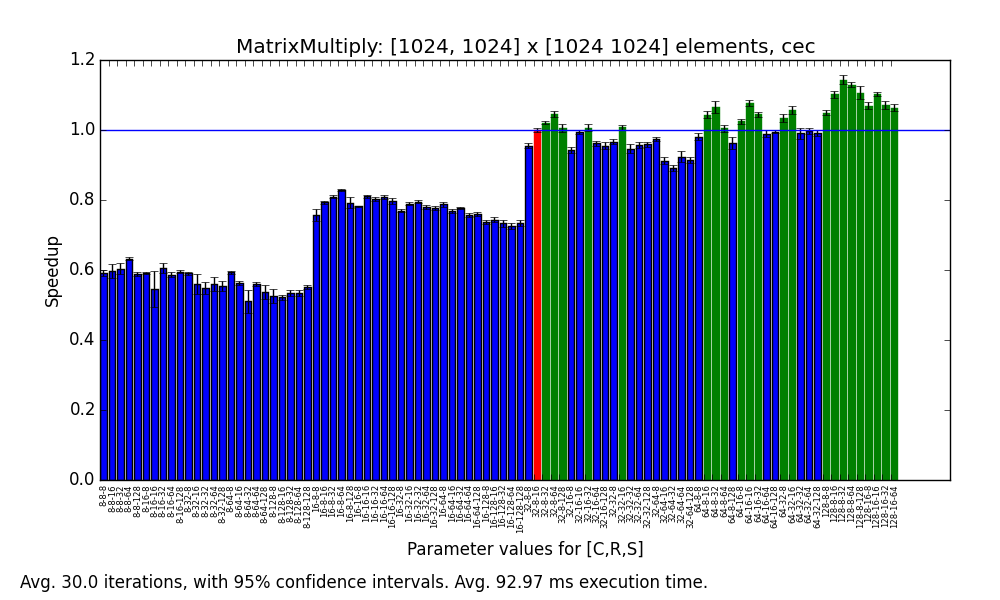
\includegraphics[width=\textwidth]{../../benchmarks/results/e2/MatrixMultiply-1024-1024-1024-cec.png}
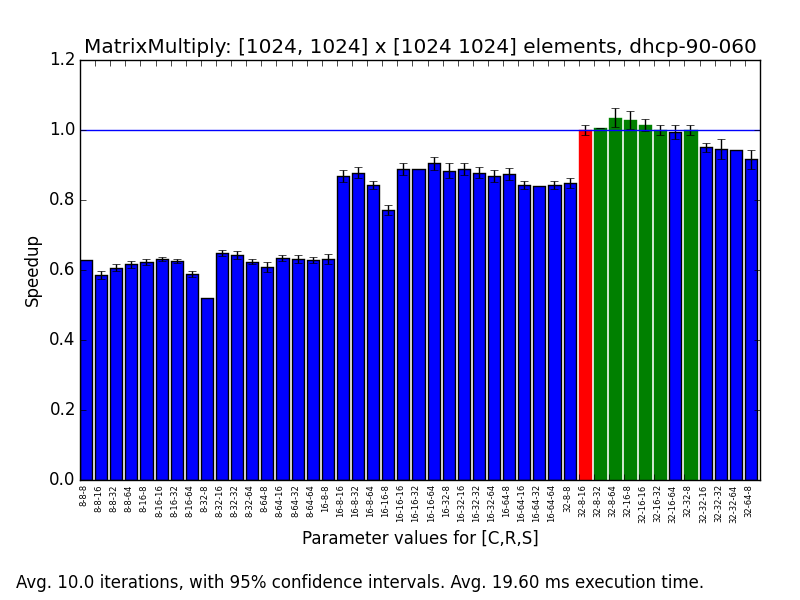
\includegraphics[width=\textwidth]{../../benchmarks/results/e2/MatrixMultiply-1024-1024-1024-dhcp-90-060.png}
\caption{Performance of Matrix Multiply kernel using different
  parameter values for the AllPairs skeleton. Optimal values for the
  CPU (top) are 128-8-64. Optimal values for the GPU are 32-8-64.}
\label{fig:mm}
\end{figure}

\begin{figure}[h]
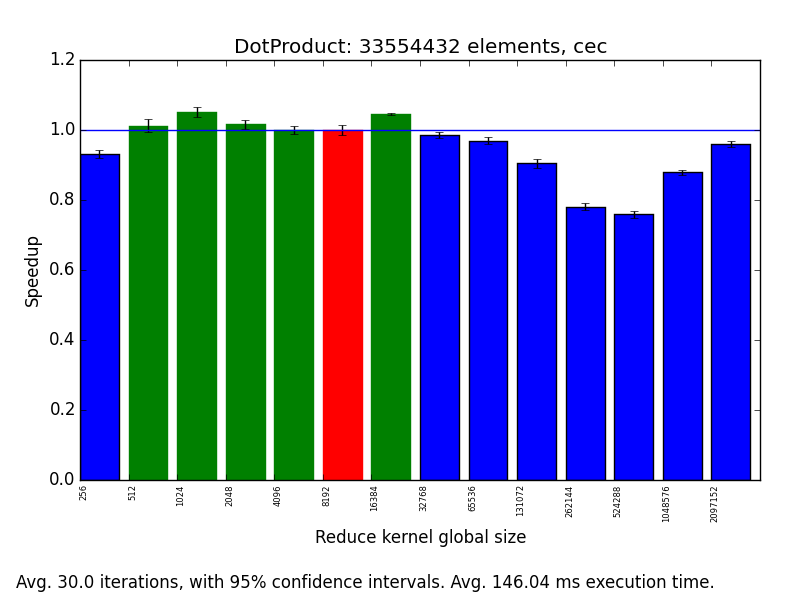
\includegraphics[width=\textwidth]{../../benchmarks/results/e3/DotProduct-33554432-cec.png}
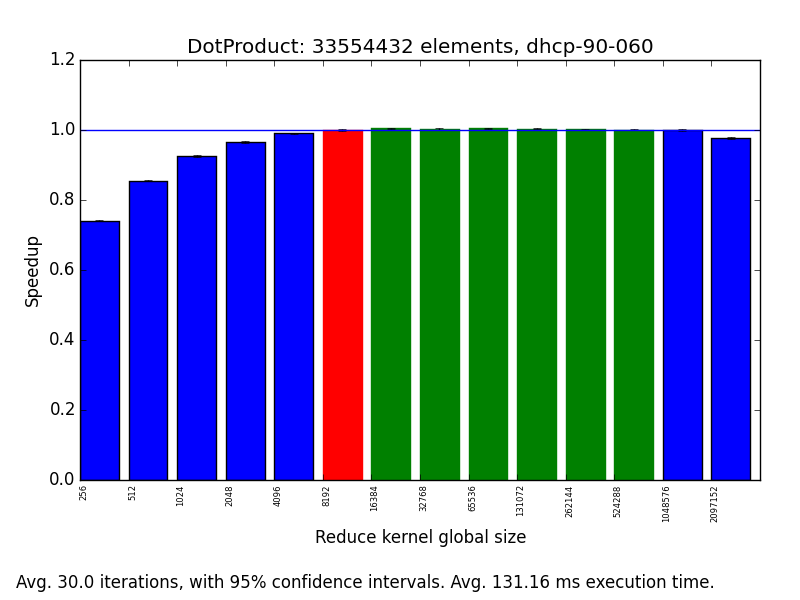
\includegraphics[width=\textwidth]{../../benchmarks/results/e3/DotProduct-33554432-dhcp-90-060.png}
\caption{Performance of Dot Product kernel using different parameter
  values for the Reduce skeleton.} % TODO: shit results
\label{fig:dp}
\end{figure}

\begin{figure}[h]
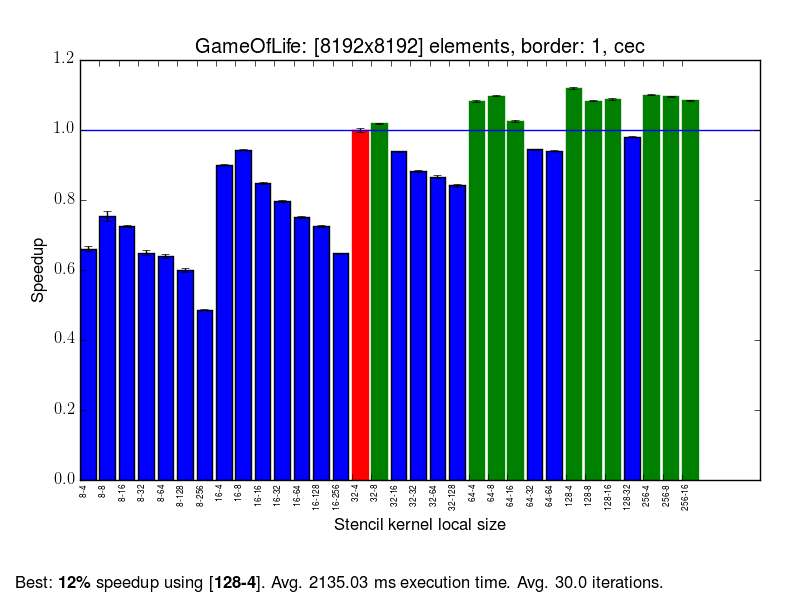
\includegraphics[width=\textwidth]{../../benchmarks/results/e4/GameOfLife-00008192-01-cec.png}
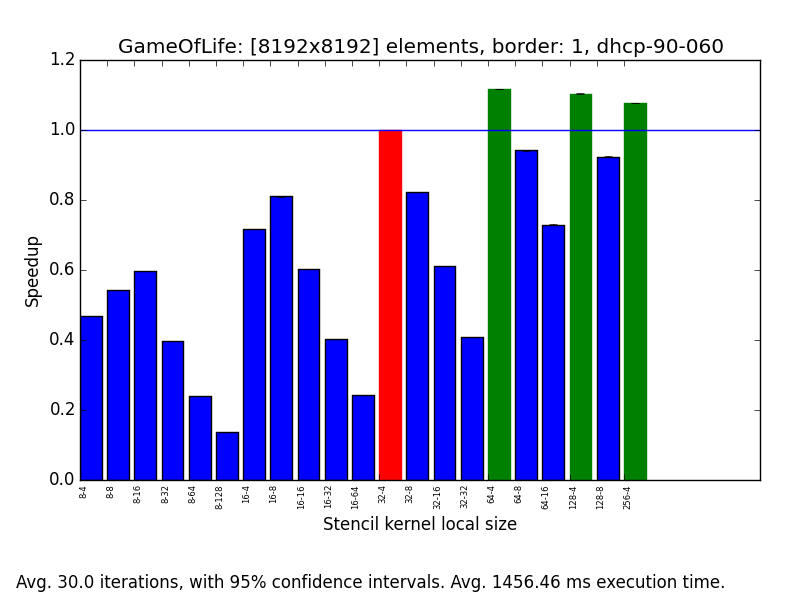
\includegraphics[width=\textwidth]{../../benchmarks/results/e4/GameOfLife-00008192-01-dhcp-90-060.png}
\caption{Performance of Game of Life using different work group
  sizes.}
\label{fig:gol}
\end{figure}

\subsection{Experimental setup}

Table~\ref{tab:hw} lists the testing hardware.

A fixed sample size of 30 is used.  Preliminary results show stable
performance for kernel execution times $\ge$ 20ms. Speedup is measured
relative to the existing values in SkelCL's public branch.

\begin{table}
\footnotesize
\centering
\begin{tabular}{| l | l | l | l |}
\hline
\textbf{CPU} & \textbf{Memory} & \textbf{GPU}\\
\hline
Intel i7-4770 & 16GiB & NVIDIA GTX TITAN\\
Intel i7-2600K & 16GiB & NVIDIA GTX 690\\
Intel i7-2600K & 8GiB & 2$\times$ NVIDIA GTX 590\\
Intel i7-3820 & 8GiB & 2$\times$ AMD Tahiti 7970\\
Intel i5-4570 & 8GiB & -\\
\hline
\end{tabular}
\caption{Testing hardware.}
\label{tab:hw}
\end{table}

% TODO: derive throughput in FLOPS

\begin{table}
\footnotesize
\centering
\begin{tabular}{| l | l |}
\hline
\textbf{Name} & \textbf{Notes}\\
\hline
Total runtime & Runtime of entire benchmark application\\
Kernel compilation time & Could influence cost/benefit analysis\\
Kernel time & Time between enqueing kernel and kernel completed\\
Data upload time & Host $\rightarrow$ Device\\
Data download time & Device $\rightarrow$ Host\\
Data sync time & Each device $\leftrightarrow$ Host\\
\hline
\end{tabular}
\caption{Measurable performance values.}
\label{tab:metric}
\end{table}

\section{Preliminary results}

Figure~\ref{fig:mm}.
Figure~\ref{fig:dp}.
Figure~\ref{fig:gol}.

\section{Related Work}

% An exhaustive search of the optimisation space for stencil benchmark
% border regions using features: PCI-type, halo size, compute
% granularity, # of GPUs. Evaluated on 2 different mobos and
% GPUs. Optimisations evaluated: rotating volume so that largest
% dimension is first dimension, adjusting halo size dynamically, and
% computing halo region first so that swap can occur concurrently with
% the rest of the computation. They concluded that the optimal setting
% depends on problem size, stencil shape GPU, and PCI. This is well
% worth studying in detail as a case of successfully applied
% autotuning to GPUs.
\cite{Lutz2013}

% * An auto-tuner which accepts as input a Fortran 95 stencil
% expression, and generates parallel implementations in Fortran, C, or
% CUDA. Targets memory bound stencil operations using 3 FDTD kernels,
% tested on 4 different architectures.
% * Does not cover performance portability across different GPUs.
% * The CUDA code generator only uses global memory (!). No
% exploitation of temporal locality.
% * Their "strategy engines" do not perform a directed search. They
% just enumerate a subset of the optimisation space, compile and run
% each option *once*, and then report the lowest time. No statistical
% certainty, no directed search.
\cite{Kamil2010}

% Dastgeer uses training data to to generate a machine-learning model
% offline, which is used at runtime to determine an execution plan
% (selecting between sequential, OpenMP, OpenCL, and CUDA back-ends)
% and parameter values for each. The paper is "first results", and
% gives no description of the machine learning techniques used, the
% training process, or the experimental method.
\cite{Dastgeer2011}

\cite{Christen2011}


\cite{Chan2009}


\cite{Collins2013}


\cite{Magni2014}

\section{Conclusions}

% TODO: extract features from kernels
% TODO: cost benefit analysis

\label{bibliography}
\printbibliography

\end{document}
